\section{Automatic Differentiation}
Evidently, training a neural network involves taking derivatives of a computation - applying the network to a batch of data to get the loss -
but how do we actually evaluate derivatives on a computer?
There are three main approaches: numerical differentiation, symbolic differentiation, and automatic differentiation (AD).
In this section, I will show how automatic differentiation is used in machine learning.

Baydin et al. \cite{Baydin2015} have an excellent survey paper on the intersection of AD and ML;
covering in more depth the pitfalls of the other techniques, both forward and reverse mode AD, how to implement AD, and the varying adoption of AD in ML libraries.
I will merely give a brief motivation of AD over the other techniques and show how backpropagation is an instance of \textit{reverse mode} AD.
I will borrow heavily from their paper.

%%%%%%%%%%%%%%%%%%%%%%%%%%%%%%%%%%%%%%%%%%%%%%%%%%%%%%%%%%%%%%%%%%
\subsection{Motivation and Overview}
Numerical differentiation refers to finite-difference methods, which evaluate the original function at two sample points and plug that into the limit definition of a derivative.
This can be highly inaccurate due to round-off and truncation errors \cite{Jerrell1997}.
It also requires sampling the function for each partial derivative required, so does not scale to the millions of parameters in a neural network.

Symbolic differentiation refers to the mechanistic application of symbolic differentiation rules to a symbolic expression tree.
This is slow and suffers from `expression swell' \cite{Juedes1991} - the rote application of rules causing the size of the derivative expression to become large and complex.

Moreover, both these techniques require the model to be defined in a closed-form expression.
This is extremely difficult for neural networks, especially in the case where the model contains control flow, common in RNNs for example.

Automatic differentiation, also known as algorithmic differentiation or just autodiff,
is a powerful family of techniques that gives evaluated derivatives, not a symbolic expression, by using pre-programmed derivatives of the individual operators applied during a computation, and the chain rule to propagate derivatives between them to get the derivative of the entire computation.
As the user code applies operators, the AD library will transparently be augmenting the values to store the derivatives too, and augmenting the operators to calculate their derivatives and propagate them to the next operators.
That is, both forward and backward functions of operators are implemented in the AD library manually.
The user runs a computation using the forward functions as usual, and the derivatives will automatically be evaluated by the AD library using the backwards functions.
The chain rule is used to compute the derivatives of a composition of operators with respect to the data at an individual operator.

This allows the evaluation of derivatives at machine precision with only a small constant factor of overhead.
Furthermore, the user can take derivatives of arbitrary, imperatively defined computations, including the use of control flow, with zero extra effort; rather than deriving complicated closed-form expressions.
This flexibility has made AD a popular tool in many fields, from machine learning to structural mechanics \cite{Haase2002}.

AD should sound a lot like backpropagation.
We run a series of forward operations, and need to compute derivative of the output of the entire computation with respect to the data at each operator. We know the derivatives functions of each operator, and take the overall derivative by using the chain rule. Backpropagation, then, is a specific instance of AD.

Specifically, backpropagation works best with what is known as \textit{reverse mode} AD, as opposed to \textit{forward mode}.
Though I will not cover the latter here, suffice it to say that forward mode allows you to take the derivative of any number of outputs with respect to a single input in only one pass.
However, it requires a separate pass for each input.
Reverse mode is the other way around -
it can take the derivative of a single output with respect to any number of inputs in one pass.
This is what happens in backpropagation -
we take the derivative of the loss with respect to a large number of parameters.
Thus, backpropagation is best implemented using reverse mode.

%%%%%%%%%%%%%%%%%%%%%%%%%%%%%%%%%%%%%%%%%%%%%%%%%%%%%%%%%%%%%%%%%%
\subsection{Reverse Mode AD}
In reverse mode automatic differentiation, a forward and backward pass occurs.
In the forward pass, as each operator is applied, the reverse dependencies are recorded.
Then, in the backward pass, the derivatives of the final output with respect to each operator output are calculated by propagating derivatives back from the output to the input using the chain rule.

In the AD literature, the forward outputs are known as the primals, and the backwards as the adjoints.
A specific forward pass on some data is a primal trace, and the backward an adjoint trace.

\begin{figure}[tb]
    \centering
    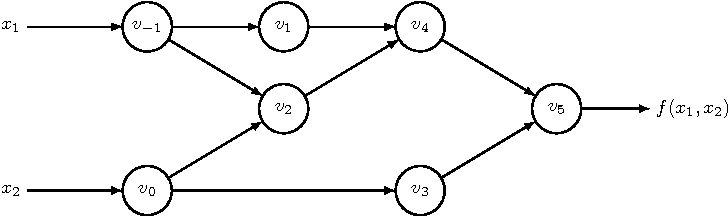
\includegraphics[width=0.75\linewidth]{rv-ad-comp-graph.png}
    \caption{Computational graph of the example \(f(x_1, x_2) = \ln(x_1) + x_1x_2 - \sin(x_2)\). See Figure \ref{fig:2-rv-ad-comp-graph} for the definitions of the intermediate variables \(\nu_{-1}\ldots\nu{5}\). \cite[Figure~3]{Baydin2015}}
    \label{fig:2-rv-ad-comp-graph}
\end{figure}
\begin{figure}[tb]
    \centering
    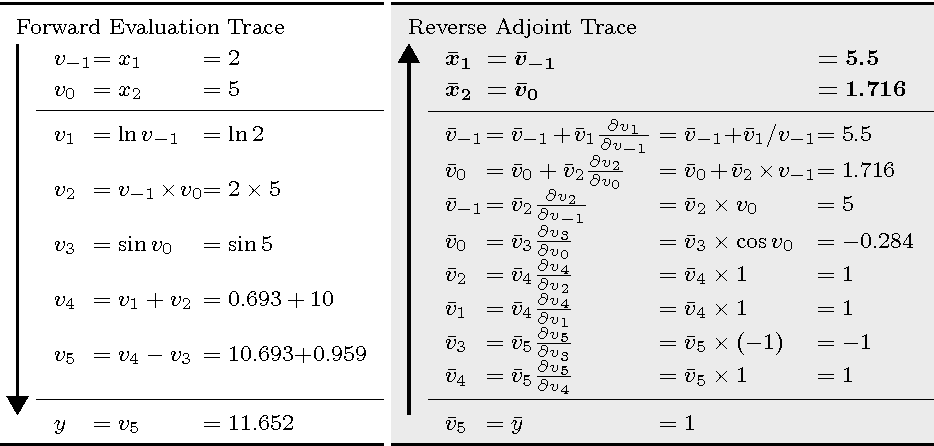
\includegraphics[width=0.9\linewidth]{rv-ad-trace.png}
    \caption{Reverse mode AD example, with \(f(x_1, x_2) = \ln(x_1) + x_1x_2 - \sin(x_2)\) at \(x_1, x_2) = (2, 5)\). After running the original forward run on the left, the augmented AD operations on the right are run in reverse. \cite[Table~3]{Baydin2015}}
    \label{fig:2-rv-ad-trace}
\end{figure}

Consider \(f(x_1, x_2) = \ln(x_1) + x_1x_2 - \sin(x_2)\).
The computational graph for this is given in Figure \ref{fig:2-rv-ad-comp-graph}.
The \(\nu_i\) denote the intermediate outputs (primals).
As the forward pass occurs, the primals are stored for use in the backward pass, and the reverse dependencies are stored.
The backward pass is initialised by setting the partial derivative of the output with itself to \(1\).
Then, we can work backwards using the chain rule.
For example, the subset of the trace computing the derivative for \(\nu_0\) will use the following rules:
\begin{align*}
    \bar{\nu_5} \;&=\; \frac{\partial \nu_5}{\partial \nu_5} \;&&=\; 1 \\[0.5em]
    \bar{\nu_4} \;&=\; \frac{\partial \nu_5}{\partial \nu_4} \;&&=\; \bar{\nu_5}\frac{\partial \nu_5}{\partial \nu_4} \\[0.5em]
    \bar{\nu_3} \;&=\; \frac{\partial \nu_5}{\partial \nu_3} \;&&=\; \bar{\nu_5}\frac{\partial \nu_5}{\partial \nu_3} \\[0.5em]
    \bar{\nu_2} \;&=\; \frac{\partial \nu_5}{\partial \nu_2} \;&&=\; \bar{\nu_4}\frac{\partial \nu_4}{\partial \nu_2} \\[0.5em]
    \bar{\nu_0} \;&=\; \frac{\partial \nu_5}{\partial \nu_0} \;&&=\; \bar{\nu_2}\frac{\partial \nu_2}{\partial \nu_0} \,+\, \bar{\nu_3}\frac{\partial \nu_3}{\partial \nu_0}
\end{align*}
An example primal and adjoint trace is given in Figure \ref{fig:2-rv-ad-trace}.

This shows how backpropagation is a specific instance of the more generic reverse mode AD.
It also shows how, in a single pass, the derivative of a single output with respect to \textit{every} intermediate variable can be calculated.

Note that the intermediate outputs were all stored during the forward pass, so they could be reused in the backward pass.
This linear space complexity (with respect to the number of operators) causes the high peak memory requirement of backpropagation.
This will be analysed in more depth in Section \ref{sec:2-4-memory-analysis}.
